% Methods Section

\section{Methodology}

\begin{frame}{Experimental Design}
\begin{center}
\begin{tikzpicture}[node distance=2cm, auto]
    % Define styles
    \tikzstyle{process} = [rectangle, minimum width=2.5cm, minimum height=1cm, text centered, draw=black, fill=blue!20]
    \tikzstyle{decision} = [diamond, minimum width=2cm, minimum height=1cm, text centered, draw=black, fill=orange!20]
    \tikzstyle{data} = [ellipse, minimum width=2cm, minimum height=1cm, text centered, draw=black, fill=green!20]
    \tikzstyle{arrow} = [thick,->,>=stealth]
    
    % Nodes
    \node [data] (input) {Legal Documents};
    \node [process, below of=input] (preprocess) {Preprocessing};
    \node [process, below of=preprocess] (model) {BERT Fine-tuning};
    \node [process, below of=model] (explain) {Explainability Analysis};
    \node [data, below of=explain] (output) {Explainable Predictions};
    
    % Arrows
    \draw [arrow] (input) -- (preprocess);
    \draw [arrow] (preprocess) -- (model);
    \draw [arrow] (model) -- (explain);
    \draw [arrow] (explain) -- (output);
\end{tikzpicture}
\end{center}
\end{frame}

\begin{frame}{Model Architecture}
\textbf{Base Model:} BERT-base-uncased
\begin{itemize}
    \item 12 transformer layers
    \item 768 hidden dimensions
    \item 12 attention heads
    \item 110M parameters
\end{itemize}

\vspace{0.5cm}
\textbf{Fine-tuning Approach:}
\begin{itemize}
    \item Classification head for clause type prediction
    \item Learning rate: 2e-5
    \item Batch size: 16
    \item Max sequence length: 512 tokens
    \item Training epochs: 3-5
\end{itemize}
\end{frame}

\begin{frame}{Explainability Implementation}
\begin{columns}
\begin{column}{0.33\textwidth}
\begin{block}{SHAP Analysis}
\begin{itemize}
    \item TreeExplainer for ensemble methods
    \item DeepExplainer for neural networks
    \item Feature importance ranking
    \item Global \& local explanations
\end{itemize}
\end{block}
\end{column}

\begin{column}{0.33\textwidth}
\begin{block}{LIME Explanations}
\begin{itemize}
    \item Text-based lime explainer
    \item Local surrogate models
    \item Perturbation-based analysis
    \item Instance-specific insights
\end{itemize}
\end{block}
\end{column}

\begin{column}{0.33\textwidth}
\begin{block}{Attention Weights}
\begin{itemize}
    \item Multi-head attention extraction
    \item Layer-wise attention analysis
    \item Token-level importance
    \item Attention pattern visualization
    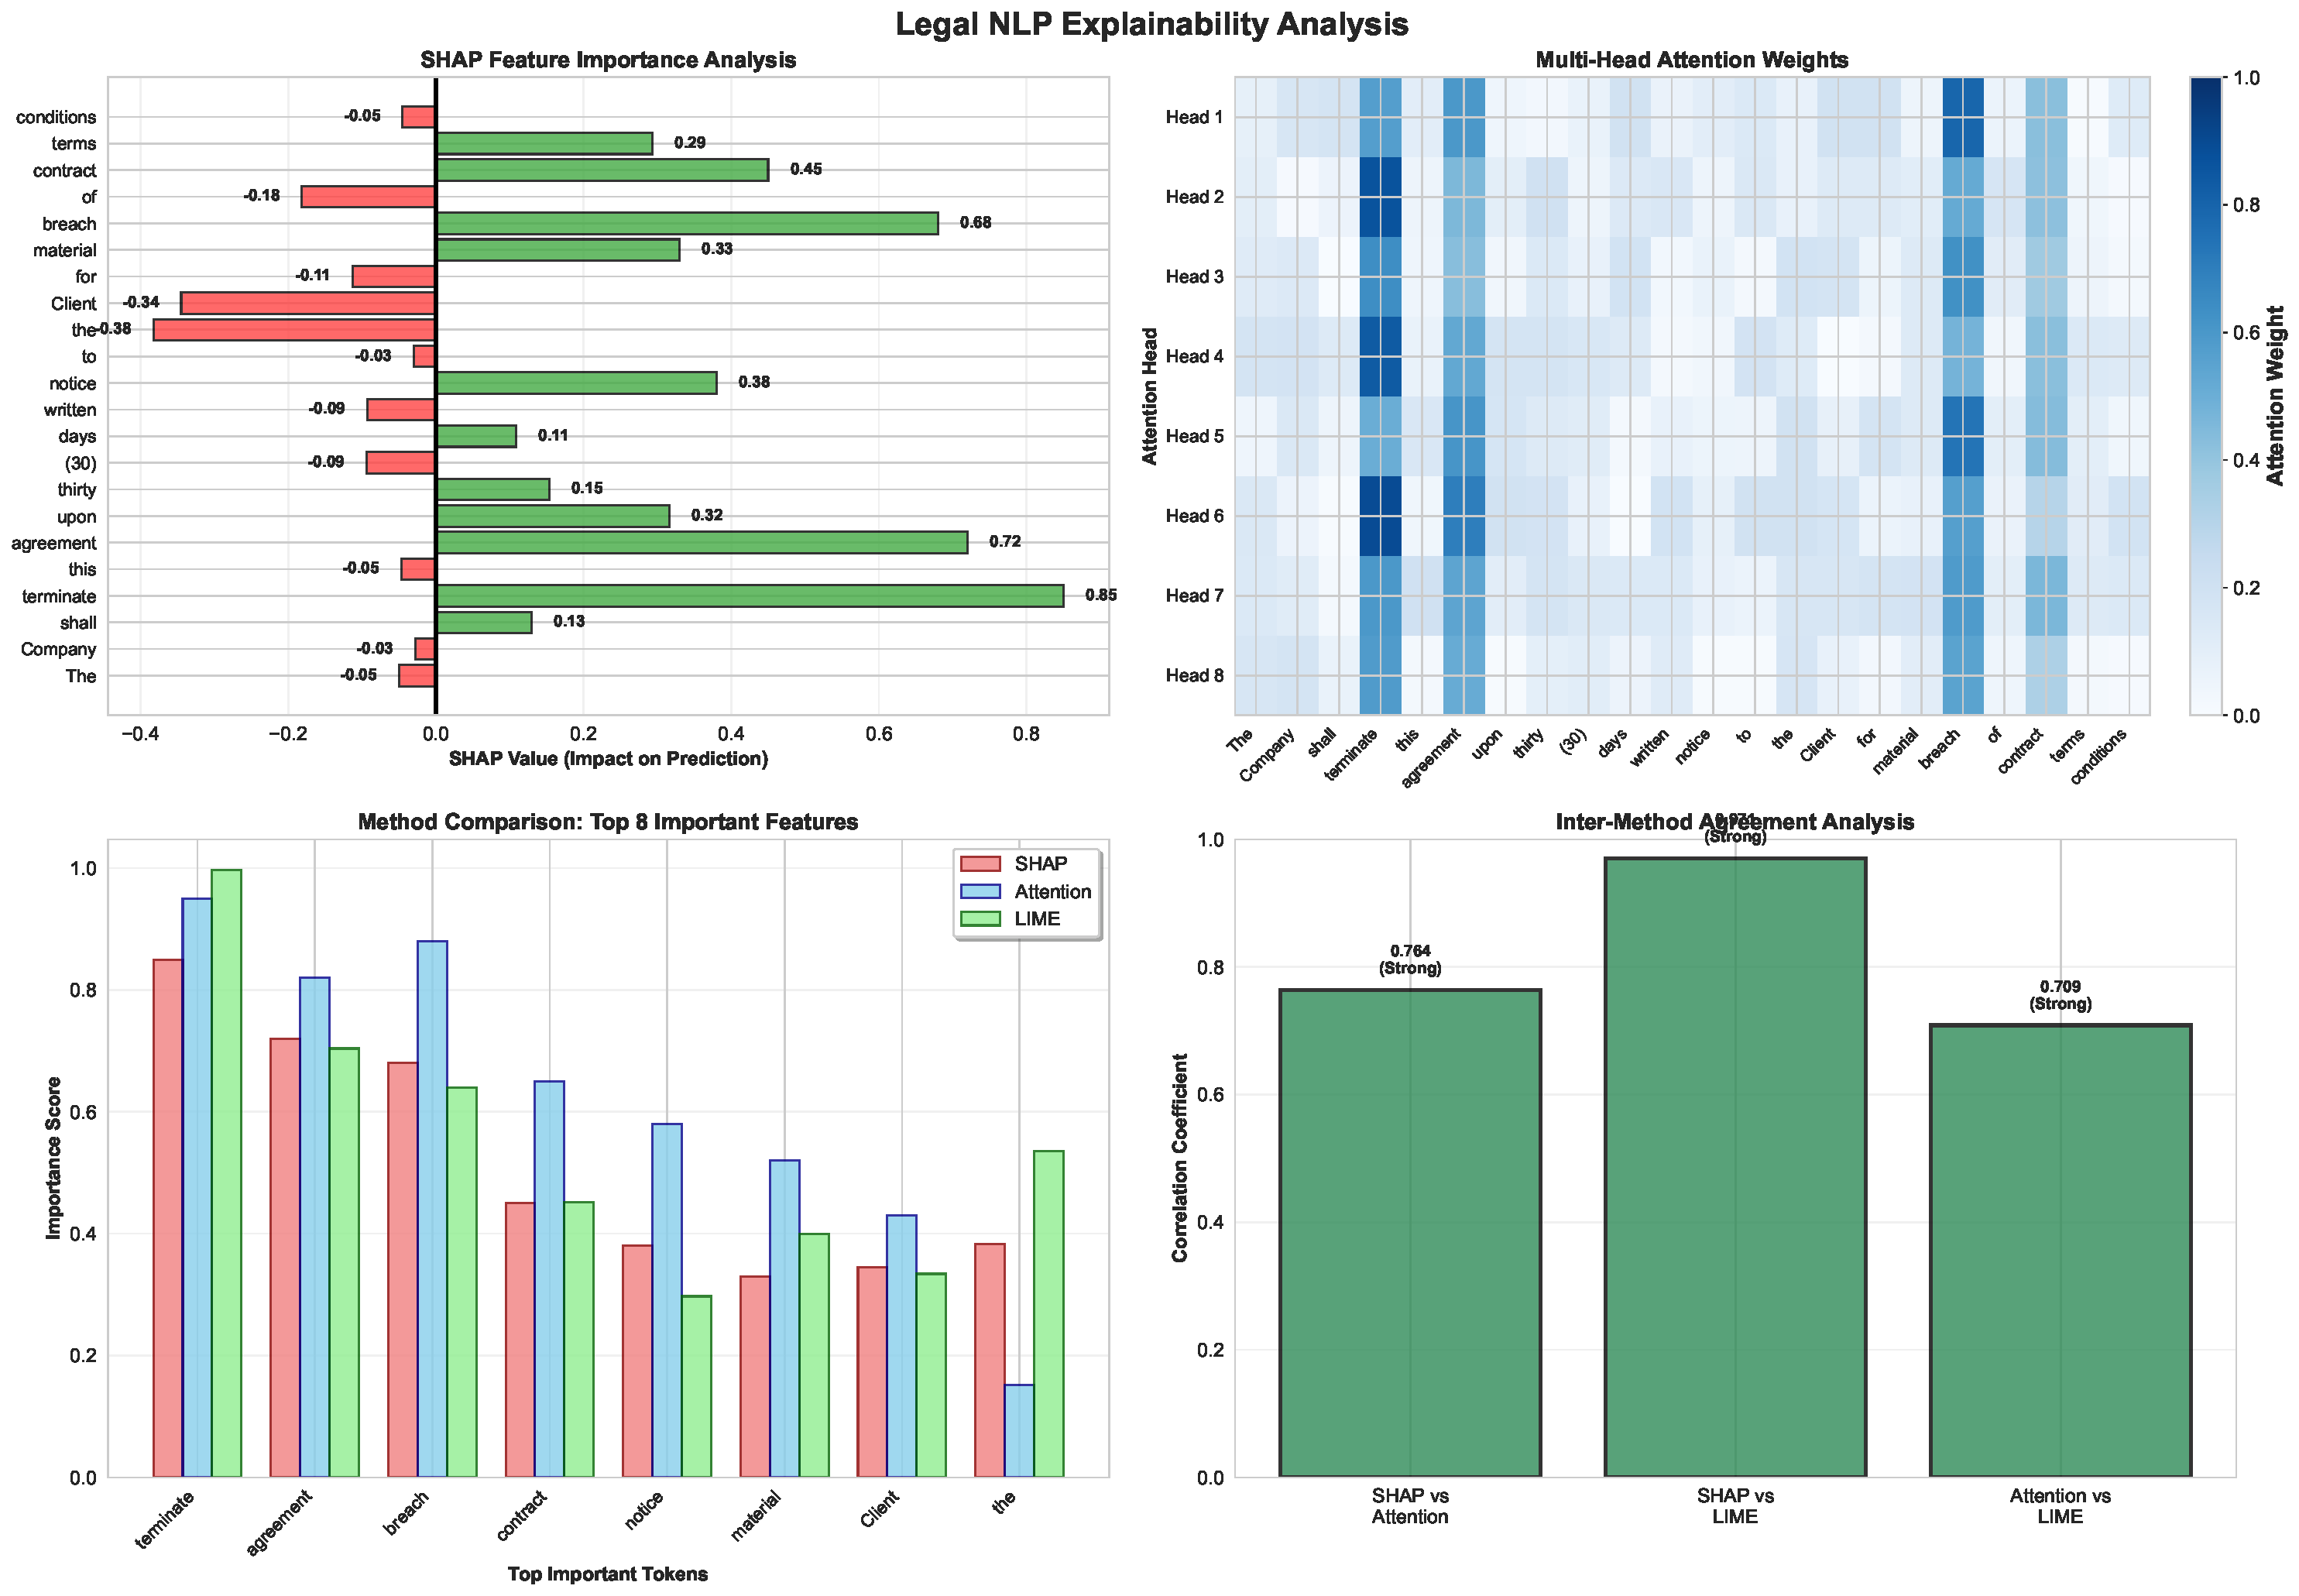
\includegraphics[width=\linewidth]{\figpath/explainability_analysis.pdf}
\end{itemize}
\end{block}
\end{column}
\end{columns}
\end{frame}

\begin{frame}{Evaluation Metrics}
\textbf{Model Performance:}
\begin{itemize}
    \item Precision, Recall, F1-score per clause type
    \item Macro and micro-averaged metrics
    \item Confusion matrix analysis
    \item Confidence score distributions
\end{itemize}

\vspace{0.5cm}
\textbf{Explainability Quality:}
\begin{itemize}
    \item \highlight{Consistency:} Agreement between methods
    \item \highlight{Faithfulness:} Correlation with model behavior
    \item \highlight{Stability:} Robustness to input perturbations
    \item \highlight{Comprehensibility:} Human-interpretable patterns
\end{itemize}
\end{frame}
